\documentclass[9pt,twocolumn,twoside]{../../styles/osajnl}
\usepackage{fancyvrb}
\usepackage{listings}
\journal{i524} 

\title{Weather Data Analysis}

\author[1]{Vishwanath Kodre}
\author[1]{Sabyasachi Roy Choudhury}
\author[1]{Abhijit Thakre}

\affil[1]{School of Informatics and Computing, Bloomington, IN 47408, U.S.A.}

\affil[1]{Corresponding authors: sabyasachi087@gmail.com, vkodre@gmail.com, athakre@gmail.com}

\dates{project-000, \today}

\ociscodes{Cloud, I524}

% replace this with your url in github/gitlab
\doi{\url{https://github.com/cloudmesh/classes/blob/master/docs/source/format/report/report.pdf}}


\begin{abstract}
The project aims to analyze any relationship between change in climate, geo- magnetic field and natural disasters with focusing on use of Hadoop Framework for data analysis and Ansible for automating deployment and monitoring.
\newline
\end{abstract}

\setboolean{displaycopyright}{true}

\begin{document}

\maketitle

\section{Introduction}

The study of environmental science and climatic changes around has been done for decades, the study
has always been predictive based on the past experiences and forecasting of the weather conditions
around us. With use of modern days technologies it determining the climatic changes and with analysis
done around it has helped human being to prepare and face the natural calamities. Though with current
equipment weather department has strengthen their arms but has not been able to be full proof and
many time its not been able to predict/ forecast the climatic changes effectively. The study of the
whether data and geo graphical changes is ongoing evolving process. Thus more and more researcher
needs modern days tools and technologies to leverage it and forecast more accurately.

\subsection{Objective}

The goal of this is to study the weather data and analyze the relationship between the geo graphical
changes such change in geo magnetic field and/or natural disaster. With use of Hadoop for distributed
data analysis aims to finds any pattern that might exists between these parameters. The course of the
analysis will also provides visualization of these parameters in order to identify any pattern in a more
intuitive way. By leveraging the power ansible for application deployment over cluster and monitoring
the application performance to determine scalability and throughput. The conclusion will be determine
by establishing any existing pattern, analysis done over it and by visualizing it.

\section{Data Sources}

Weather data has been recorded since 19th century. This data can be used to estimate climate changes
and forecasting. The same data can be can be used to find any existing pattern with natural disasters.
Following sources has been compiled for weather, natural disaster and geo magnetic fields.
\begin{itemize}
\item Weather-Data\cite{Weather-Data}
\item Natural Disaster\cite{Disaster-List-Data}
\item Geo Magnetic Field\cite{Geo-Magnetic-Data}
\end{itemize}

\section{High Level Design}

The design of the application is thought of leveraging power of Hadoop as main processing unit of
analysis with deployment on the cluster environment where application requires multiple processing
units for execution, database for persistence and visualization tools for graphical outputs.
\begin{figure}[htbp]
\centering
\fbox{\includegraphics[width=\linewidth]{images/weather_analysis_architecture}}
\caption{Architecture}
\label{Reference:false-color}
\end{figure}
The project is divided into following steps:

\begin{itemize}
\item Data cleaning and persistence - The raw data cannot be use directly for analysis. First data has to be parsed and required parameters will be extracted. Then this extracted data will be dumped into a NoSql database.
\item Core Analysis Program - Core analysis program will be responsible for figuring out any hidden patterns between aforesaid parameters. Program will compare natural disasters occurred, geo-magnetic orientation and climate data
set on a given location and duration and compute relationship between them. The program will be an
MapReduce implementation and is the heart of the application. The program will be executed through
Hadoop framework. Hadoop will execute the program in a distributed manner.
\item Deployment and Monitoring - The application needs multiple processing units and monitoring system. Ansible will be used for deployment and manage nodes for program execution.Ansible will be responsible for following tasks
i)   Deployment and configuration of Hadoop on the multiple nodes.
ii)  Starting Hadoop servers, inserting/reading data.
iii) Execution of the commands to run the analysis using Hadoop to filter the input data and write
response to HDFS or some output file.
iv)  This output can be then passes to the visualization step as the input data.
\item Visualization - Finally once the programs completes execution, using the scikit-tool or other visualization tool
kit and the output file, graphs and patterns depicting the relationship can be plotted more intuitive representation.
\item BenchMarking - The application can be benchmarked for the scalability by addition more nodes and checking the
performance for strong scaling. The report will be represented in tabular format.
\end{itemize}


\section{Data Curation}
Getting data ready is the very first and basic step for analysis. We have chose NCDC as our source of data. NCDC exposes few rest apis for accessing weather data. Following will give you a brief understanding on the apis used for getting the required data.
\begin{itemize}
\item I) Datasets : This groups data into monthly daily , yearly pattern. There are eleven different datasets. We will be choosing GSOM (Global Summary Of Monthly) as our primary datasets. (URL : https://www.ncdc.noaa.gov/cdo-web/api/v2/datasets ,Attributes : GSOM). For this project we will use GSOM only.	
\item II) Data Categories: This groups data into data category like Temperature, Pressure etc. We will consider only few. ( URL : https://www.ncdc.noaa.gov/cdo-web/api/v2/datacategories, Attributes : "TEMP" (Air Temperature) , "PRES" (Pressure) , "EVAP" (Evaporation) and "VELOCITY" (Velocity) ). For our project we will be using PRCP, SNOW, TMAX, TMIN and TAVG.
\item III) Data Types: This group Data Categories into further smaller sub types. (URL : https://www.ncdc.noaa.gov/cdo-web/api/v2/datatypes?datasetid=GSOM\&datacategoryid=TEMP , Attributes : "TAVG" (Average Temperature), "TMAX" (Maximum Temperature) and "TMIN" (Minimum Temperature)    ) Other Data Categories does not have sub type.
\item IV) Location Categories: This groups data in terms of location. (URL : https://www.ncdc.noaa.gov/cdo-web/api/v2/locationcategories , Attributes : "CITY" , "CLIM\_DIV" (Climate Division), "CLIM\_REG" (Climate Region) , "CNTRY" (Country) ,"ST" (State)). For this project we will be downloading data for India only.
\item V)  Location: Groups data in terms of country, state etc. (URL : https://www.ncdc.noaa.gov/cdo-web/api/v2/locations?locationcategoryid=CNTRY, Attributes : "FIPS:IN" (INDIA) , "FIPS:IO" (Indian Ocean))	
\item VI) Station : This collects stations details based on the location id. (URL : https://www.ncdc.noaa.gov/cdo-web/api/v2/stations?locationid=FIPS:IN , Attributes: ids , mindate and maxdate). All of the stations details will be collected.	
\item VII) 	Data : This collects actual weather data for the given stationId,
 startdate and enddate. (URL : https://www.ncdc.noaa.gov/cdo-web/api/v2/data
 ?datasetid=GSOM\&stationId=GHCND:IN1NCBC0005\&startdate=1970-10-10
 \&enddate=1971-10-10). Since the project only requires only 5 attributes, 
 further filter is applied while invoking the API. The data received will be saved into database. 
\end{itemize}

\subsection{Collecting Data}
NCDC uses token based authentication for security and with each token , no more than 10,000 hits are allowed per day. Well 10,000 seems huge but truly its not. We have targeted one country (India) and 5 attributes chiefly precipitation, snow, maximum temperature, minimum temperature and average temperature for each month. Total number of weather data stations in the country is around 3500 and each station has a data range of 30 to 50 years. This leads to a total of 100,000 hits or more. To handle this, we need to load data incrementally, i.e. the curation program should have the ability to resume the download from the last save point. Before we dive more into logical section , lets first see the technology stack for data collection.

\subsection{Technology Stack}
We have considered python , Apache thrift and Apache Hbase for data curation step. We will be covering a short introduction of the steps to configure the system, before diving into the core logic of curation. Since we are going to use Apache Hadoop for our analysis purpose, Hbase comes as a natural choice of NoSql database. Java is the default language for both Hadoop and Hbase. So now the question is how to connect to Hbase using python and the solution is Apache Thrift or thrift. Thrift is a library from apache which generates hbase client. Thrift supports many third party languages including python. The following steps will be required to install thrift first.
\subsubsection{Install Apache Thrift \cite{thrift-python-install}}
\begin{itemize}
\item 1) Download Thrift from 
"http://redrockdigimark.com/apachemirror/thrift/0.10.0/thrift-0.10.0.tar.gz".
\item 2) Extract the file and run ./configure.
\item 3) Execute sudo make install or simply make to generate the binaries.
 If using make, the thrift binaries has to put into path manually 
 (can be found under compiler/cpp/).
\item 4) After thrift is available in path , it can be tested by 
running "thrift --version".
\item 5) Then the python module has to be created to be used within python.
 To do this download "https://github.com/apache/hbase/blob/master/hbase-thrift/
 src/main/resources/org/apache/hadoop/hbase/thrift/Hbase.thrift" file.
\item 6) Then execute "thrift --gen py <path/to/Hbase.thrift>". This will 
generate "gen-py" folder.
\item 7) Add this folder to python path by export 
PYTHONPATH=<path/to>/gen-py/:\$PYTHONPATH.
\end{itemize}
For details you can check \href{https://acadgild.com/blog/connecting-hbase-with-python-application-using-thrift-server/}{Installation} steps.Installation of Hbase will be discussed later along with Hadoop.
Now thrift is ready to use. Execute "/hbase thrift start" to start the thrift server. Hbase has to be started separately.
\subsubsection{Install Happybase \cite{happybase-install}}
Happybase is a wrapper program written on thrift to facilitate data access layer in python in a more readable and swift way. Rather than using thrift client directly we will be using happybase python module. To install happybase run "pip install happybase". 
Once done test the python library by running the following test code 
\begin{lstlisting}[language=Python,caption=Connect-Hbase,breaklines=true]
import happybase as hbase				

connection = hbase.Connection('localhost')
print connection.tables()
\end{lstlisting}

\section{Hbase and Table Structure}
Hbase \cite{hbase} is a column based key-value database. We have considered two tables for weather data `wda\_stations` and `wda\_weather`. The structure of the tables are as follows\newline
\begin{lstlisting}[label=JSON,caption=WDA\_STATIONS Table,breaklines=true]
[{station-id-key : {
	station : {name : {} , id : {}},
	date_range : {
		min_date : {} ,
		max_date : {}
	 },
	location : {
		latitude : {},
	 	longitude : {}
	}
}}]
\end{lstlisting}
\begin{lstlisting}[label=JSON,caption=WDA\_WEATHER Table,breaklines=true]
[{yyyy-mm-key : {
	weather : {station-id : {
		data-type : {value}			
}}}}]
\end{lstlisting}
\subsection{Table Definition}
Stations table will consist of all the weather stations with its location and the date range within which it is was active. Location will have the latitude and longitude. The station id will be the key for the table. NCDC uses a uniquely identifiable key for the stations across the globe. This makes the best attribute for the primary key irrespective of country and region. Weather table is a more completed table and has dynamic column family. The key for the table is the year and month in (YYYY-MM) format. Each key contains all the stations with their weather parameter. For example say a key 1967-01 (meaning January 1967) is having 10 stations with station id sid-1 to sid-10. Each station id will having 4 parameters or data types (TAVG,TMAX,TMIN and PRCP). And finally each parameter have their values. 

\section{Data Persistence Layer}
The project is structured with python packages. We have a specific package for persistence as 'iu.i524.S17IRP013.dao'. The dao has the scripts to connect hbase and performs db operations. The base script is `hbase\_connect.py` which does the connection. The connection is made through Apache Thrift Rest Api. It has the connection object , which is used by the other two dao classes.

\subsection{Station Dao}
This script does all CRUD operations on stations table. On startup it will create the table if not available. It has 2 main functions insert and retrieve. The insert function takes key value pair as argument and put it into hbase table. Another function and the important one is `get\_station\_data` which takes the start row as argument and returns next ten records. This is done via scan command of hbase which supports record limitation.
\begin{lstlisting}[language=Python,caption=Stations Dao,breaklines=true]
def get_station_data(start_row=''):   
    st_list = dict()
    count = 0    
    if(start_row == ''):    
        for key, data in table.scan(limit=10):
            st_list[key] = {'min_date':data['date_range:min_date'], 'max_date':data['date_range:max_date'] , \
                            'station_id': data['station:id'], \
                            'latitude':data['location:latitude'], \
                            'longitude':data['location:longitude']}            
    else:
        for key, data in table.scan(limit=11, row_start=start_row):            
            count = count + 1
            if(count > 1):
                st_list[key] = {'min_date':data['date_range:min_date'], 'max_date':data['date_range:max_date'], \
                            'station_id': data['station:id'], \
                            'latitude':data['location:latitude'], \
                            'longitude':data['location:longitude']}    
    return st_list
\end{lstlisting}
\subsection{Weather Dao}
Weather dao is similar to station in dao in all respect except it deals with weather table. Apart from the getting records from the weather table, there is another method to get all keys from the table. We will see in later sections why we need the entire key list from the table.


\section{Weather Data Persistence}
Once happybase, thrift and hbase is functional, we are ready to download our weather data. Weather data download is divided into two steps 1) Getting weather stations details for a given country and 2) Getting Weather data for a given station. Lets see them individually :
\begin{itemize}
\item Download Weather Stations - To consume rest services we have used python's inbuilt request response module.  Let us walk you through the code. We have two main python script one for data access and another for rest consumption. "stations\_dao.py" is for accessing table "wda\_stations" in hbase. The functions are self explaining and hence will not be repeated here. "weather\_services.py" is for consuming NCDC rest services. To load all stations , we will be using the code \textit{`FIPS:IN`} i.e the region code for India.\newline

\begin{lstlisting}[language=Python,caption=Get Weather Stations,breaklines=true]
def get_stations(country='FIPS:IN', offset=0):
    url = NCDC_API + NCDC_SERVICES.STATIONS + \
    '?locationid=' + country + '&offset=' + str(offset)
    
    response = requests.get(url, headers=HEADERS)
    return response.json()

def load_stations():
    limit = 25    
    offset = 0
    nbr_of_records = 0
    result = Services.get_stations(offset=offset)   
    while(result != {}):       
        nbr_of_records = nbr_of_records \
        + insert_station(result['results'])
        offset = offset + limit
        result = Services.get_stations(offset=offset)
    print str(nbr_of_records) \
    + ' stations loaded successfully !!'    
\end{lstlisting}
The function `load\_stations` calls `get\_stations` till all the available stations are downloaded. `insert\_station` is the \textit{DAO (Data Access Object)} call and inserts the dataset into hbase table.

\item Download Weather Data - With all stations in the table, we invoke the data api of NCDC for downloading weather data. The argument for getting weather data is station id and date range. The two main methods for loading weather data are as follows 

 \begin{lstlisting}[language=Python,caption=Get Weather Stations,breaklines=true]
def load_weather_data():
    start_row = ''
    st_list = stations.get_station_data(start_row=start_row)
    while st_list != {}:
        for key, value in st_list.items():
            get_weather_data(startDate=value['min_date'], \
            endDate=value['max_date'], stationId=key, station_details=value) 
            start_row = key
        print 'Weather Data loaded till station id = ' + key
        st_list = stations.get_station_data(start_row=start_row)    

def get_weather_data(station_details, startDate='1968-01-01', endDate='1970-01-01', stationId='GHCND:IN001011001'):
    date_range_list = AppUtil.get_year_list(start_date=startDate, end_date=endDate)
    for date_range in date_range_list:
        limit = 25    
        offset = 0
        result = Services.get_weather_data(startDate=date_range['min_date'],\ endDate=date_range['max_date'], stationId=stationId, offset=offset)   
        while(result != {}):        
            # print result['results']
            insert_result(result['results'], station_details)
            offset = offset + limit
            result = Services.get_weather_data(startDate=date_range['min_date'],\ endDate=date_range['max_date'], stationId=stationId, offset=offset)

\end{lstlisting}

The `load\_weather\_data` function retrieves station data from the station table in a batch of ten. For each station id, it is then passed to `get\_weather\_data` function to get weather data for the given station id. This data is again persisted into wda\_weather table for future analysis and usage. These are the main functions to download weather data. All other functions are helper functions to enable the download. 

\end{itemize}


\section{Install Python Program}
Our python programs are structure and packaged. So to use it, we need to install the packages , in order to make them available in the classpath or pythonpath. There is a setup.py script provided with the main source folder. This script installs the entire package into python core folder. To execute this \textit{pip} must be pre-installed. Once pip is available run the following command 

\begin{lstlisting}[language=Python,caption=Install python packages,breaklines=true]
sudo pip install  <path_to_src_folder>/src
\end{lstlisting}

Use sudo or super user to install as other may have permissions issues. Once they are installed , we are ready to run our map reduce program.

\section{Execution}
The application expects all the data in hbase are prefetched and ready. For downloading the datasets into hbase follow the steps 
\begin{itemize}

\item Install the python packages. Check all installations hbase, hadoop , thrift and happybase.
\item Start Hadoop and Hbase and Apache Thrift.
\item Open up python cli and run the command  `iu.i524.S17IRP013.hadoop.init.DataSetup.py`.
\item The above command will take time and will dump data into hbase table.
\item It also created hdfs input folder as '/wda/input' and write `wda\_row\_keys.txt` file into it. This file will have all the keys (year-month format) from weather table.  

\end{itemize}

\subsection{Run MapReduce}
We need hadoop streaming api to execute our ma reduce program. Hadoop streaming api reads from hdfs and write it onto the standard io. This data is then read by our map program \textit{wda\_mapper.py} and further sent to reducer program \textit{wda\_reducer.py}.
\begin{lstlisting}[language=bash,caption=Run MapReduce,breaklines=true]
bin/hadoop jar <path_to_streaming_jar>{share/hadoop/tools/lib}/hadoop-streaming-2.7.3.jar \
-file <path_to_mapper>/run/wda_mapper.py -mapper wda_mapper.py \
-file <path_to_reducer>/run/wda_reducer.py -reducer wda_reducer.py \
-input /wda/input -output /wda/output
\end{lstlisting}
The above will  execute the map reduce analysis program and write the output into hdfs `/wda/output` folder. Once the program is finished check the output with following command :
\begin{lstlisting}[language=bash,caption=Run MapReduce,breaklines=true]
hdfs dfs -ls /wda/output
hdfs dfs -cat /wda/output/<name_of_the_file>{part-r-00000}
Output >>
{'TAVG': ('GHCND:IN001020700', '35.02'), 
'TMAX': ('GHCND:IN001020700', '43.08'), 
'PRCP': ('GHCND:IN001011000', '863.7'), 
'TMIN': ('GHCND:IN001020700', '14.08')}
\end{lstlisting}

\section{Benchmarking}
The aforesaid program has been executed on futuresystems. The execution time has been collected by increasing nodes from 1 (single) to 3 (multiple) with 2cpus each. 
\begin{figure}[htbp]
\centering
\fbox{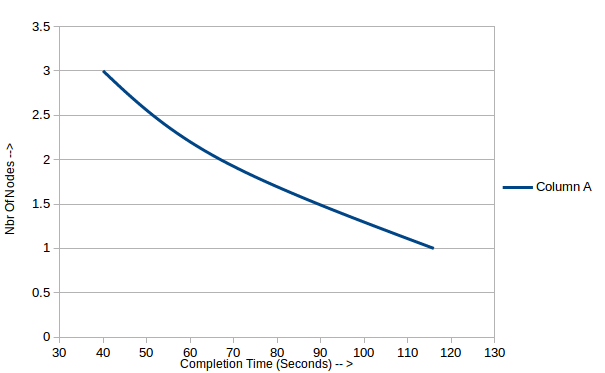
\includegraphics[width=\linewidth]{images/graph}}
\caption{Benchmarking}
\label{Reference:false-color}
\end{figure}
The graph indicates the reduction in time with increase in nodes. Since the data used for the sample is not big enough , the time taken for starting the framework is considerably high as compared to total time taken by the analysis program itself.
\begin{figure}[htbp]
\centering
\fbox{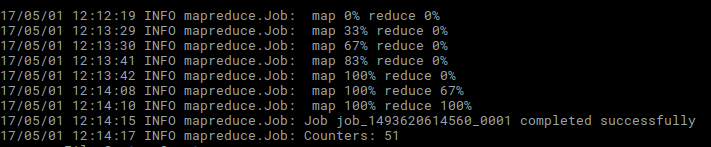
\includegraphics[width=\linewidth]{images/MR_Benchmark_fs}}
\caption{Map Reduce Snapshot}
\label{Reference:false-color}
\end{figure}
So only the map reduce time or the program time has been considered and not the ancillary time which includes time to start the hadoop framework. 

\section{Scope of Extensions}
The application is only distribute the data load from the hbase table. But fetching data from NCDC is sequential. Though its only a one time job , it takes considerable amount of time to download. The same application can be extended to use Hadoop MapReduce for downloading and persisting the raw data from Rest APIs. The same fundamentals can be used for this purpose. Initial weather stations can be downloaded sequentially and then the keys are to be distributed in HDFS for further weather data download. 
\subsection{Limitation}
There is a limitation in download imposed by NCDC. NCDC uses token bases authentication which allows only 10000 invocation per day. To distribute the download among multiple nodes requires multiple tokens.

\section{Conclusion}
MapReduce (MR) with Hadoop is an efficient framework for distributed computing. It can be run on any commodity hardwares and virtual machines. It has also some useful plugins available for shared computing which can share dataset without doing any IO operations,ex - Twister and Spark. Python with Hadoop on other hand is not so great combination as the communication requires additional layer i,e Standard IO. We have seen earlier that there is no support for Hbase communication within the hadoop as well. FutureSystems and Jetstream works well with the framework. Chameleon VMs did not have all ports opened (except 22 for ssh) which is a must for Hadoop to work in cluster as Hadoop uses IPC protocol for inter node communication. 

\section{Deployment Using Ansible}

Ansible is open source automation tool. It can be used for deployment of software, configuration  management and automation in the execution of application. 
It also serves for monitoring of the state of the application. As per current state of our project we have used ansible for deployment of software in our project. 
The script deploys Java, Hadoop, Hbase on the independent clusters. It also configures the properties in the key files. 

\subsection{Inventory Configuration}

Inventory file contains the list of hostname or nodes that can be accessible by ansible. These nodes are then used in the script for deployment and configuration. 
In the current project chameleon server nodes were created and configured. These IP address can be changed dynamically. This file can also contain the group inside 
Which multiple ip can be configured.

[weatherCluster]
129.114.33.165 ansible\_ssh\_user=cc
129.114.33.179 ansible\_ssh\_user=cc
129.114.33.109 ansible\_ssh\_user=cc

\subsection{Playbook}

Playbook works on mentioned host of group. It mentions the roles those will be operated on each of the host. The main.yml  inside the task folder within each roles will be applied to 
The cluster. 

---
- hosts: weatherCluster 
  remote\_user: root
  roles:
    - master
    - hadoop
    - hbase
    — hdfs

\subsection{Roles}

% Bibliography

\bibliography{references}
 


\end{document}
